\section{Ασύμμετρη κρυπτογραφία} \label{section:2-2-asymmetric-cryptography}

Η ασύμμετρη κρυπτογραφία (asymmetric cryptography) ή κρυπτογραφία δημόσιου κλειδιού (public-key cryptography) αποτελεί κρυπτογραφικό σύστημα που βασίζεται στη χρήση ενός ζεύγους κλειδιών (key pair), του \textit{δημόσιου} (public key) και του \textit{ιδιωτικού} (private key). Αυτά τα κλειδιά είναι μαθηματικά συνδεδεμένα ως εξής:

\begin{itemize}
	\item Το ιδιωτικό κλειδί δε μπορεί να προκύψει γνωρίζοντας το δημόσιό του
	\item Ό,τι κρυπτογραφηθεί από το ένα μπορεί να αποκρυπτογραφηθεί μόνο από το άλλο 
\end{itemize}
	
Η δημιουργία ενός ζεύγους κλειδιών επιτυγχάνεται μέσω μιας \textit{γεννήτριας κλειδιών} (\textenglish{key generation function}), η οποία χρησιμοποιεί ειδικούς αλγορίθμους (π.χ. RSA), δεχόμενη ως είσοδο έναν τυχαίο αριθμό. Από τα παραχθέντα κλειδιά, το δημόσιο γνωστοποιείται σε τρίτους, ενώ το ιδιωτικό παραμένει μυστικό.

\begin{figure}[H]
	\centering
	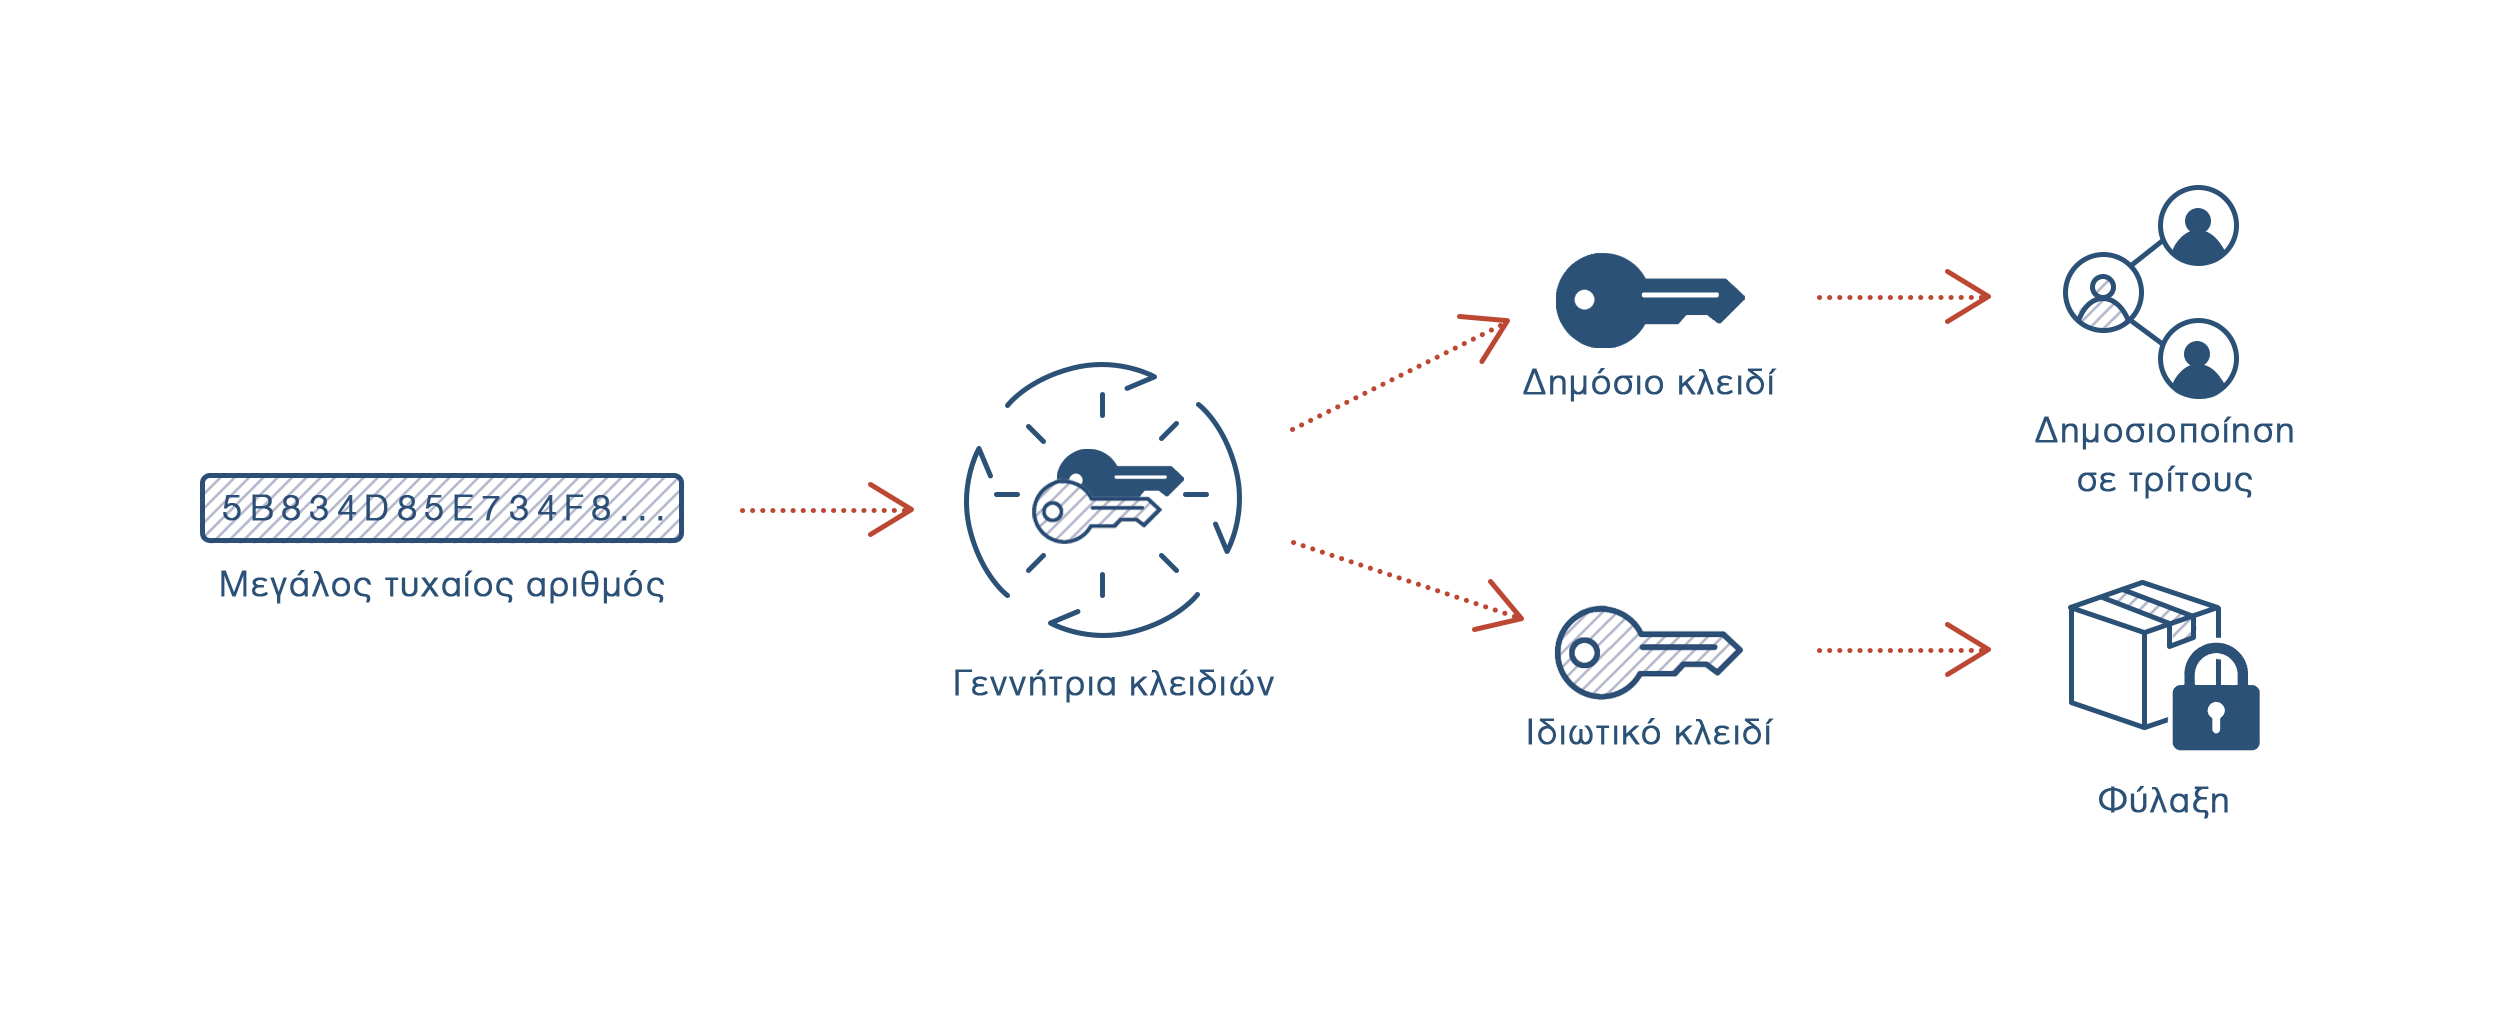
\includegraphics[width=15cm]{assets/figures/asymmetric-key-generation.png}
	\caption{Παραγωγή ασύμμετρου ζεύγους κλειδιών}
\end{figure}

Ο χρήστης μπορεί να χρησιμοποιήσει τα κλειδιά για δύο βασικούς σκοπούς:

\begin{enumerate}
	\item Για να αποκρυπτογραφήσει μηνύματα άλλων χρηστών, οι οποίοι τα κρυπτογράφησαν χρησιμοποιώντας το δημόσιο κλειδί του. Με αυτόν τον τρόπο εξασφαλίζεται η \textit{εμπιστευτικότητα} (confidentiality).
	\item Για να υπογράψει ψηφιακά ένα μήνυμα, κρυπτογραφώντας το hash των δεδομένων του με το ιδιωτικό του κλειδί. Έτσι, ο παραλήπτης του μηνύματος μπορεί μέσω της ληφθείσας \textit{ψηφιακής υπογραφής} (digital signature):
	\begin{enumerate}
		\item Να επαληθεύσει την ταυτότητα του αποστολέα, αποκρυπτογραφώντας επιτυχώς την ψηφιακή υπογραφή με το δημόσιο κλειδί του τελευταίου. Εξασφαλίζεται έτσι η \textit{πιστοποίηση} (authenticity) της προέλευσης των δεδομένων.
		\item Να επιβεβαιώσει ότι το μήνυμα έφτασε αναλλοίωτο, εφόσον το hash των δεδομένων συμπίπτει με το hash εντός της ψηφιακής υπογραφής. Με αυτόν τον τρόπο εξασφαλίζεται η \textit{ακεραιότητα} (integrity) των δεδομένων.
	\end{enumerate}
\end{enumerate}

Με τον συνδυασμό των παραπάνω, λέμε ότι δύο χρήστες μπορούν να επικοινωνούν μεταξύ τους με \textit{κρυπτογράφηση απ' άκρη σ' άκρη} (end to end encryption).

\begin{figure}[H]
	\centering
	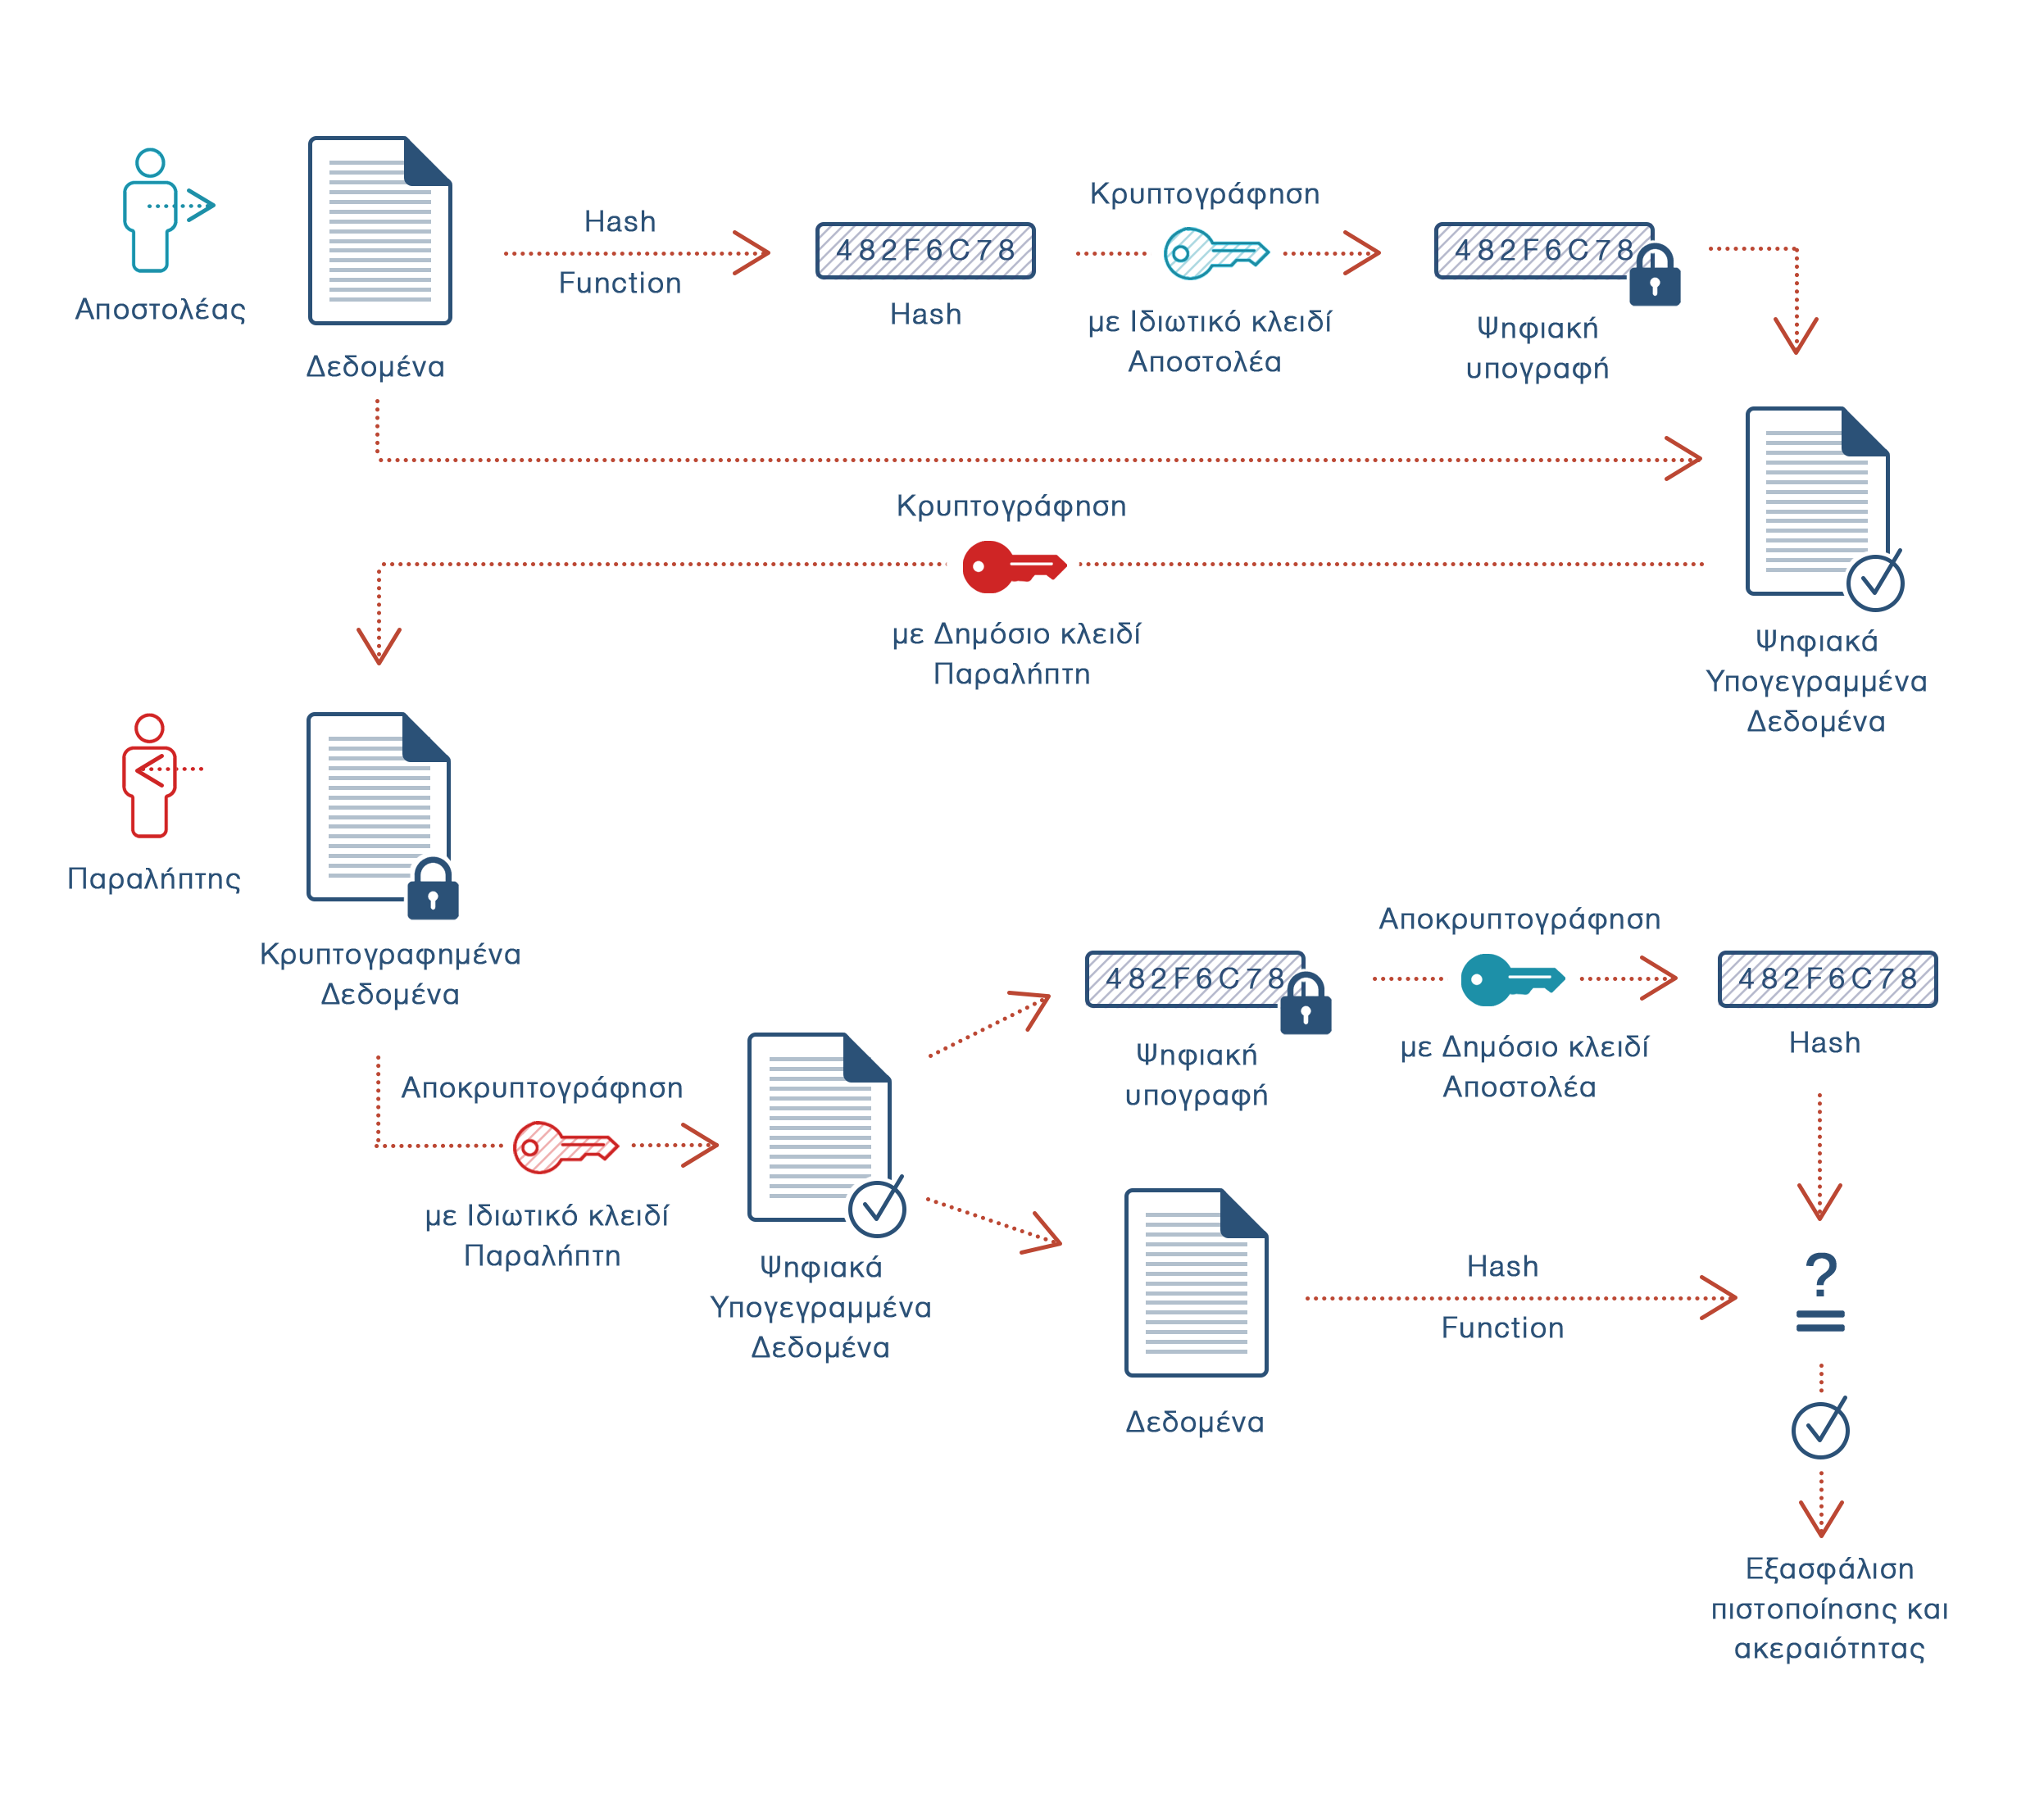
\includegraphics[width=15cm]{assets/figures/asymmetric-end-to-end-communication.png}
	\caption{Κρυπτογράφηση απ' άκρη σ' άκρη}
\end{figure}

 Μία προσέγγιση στην κρυπτογραφία δημόσιου κλειδιού είναι η κρυπτογραφία ελλειπτικής καμπύλης (Elliptic-Curve Cryptography ή ECC). Η ECC βασίζεται στην αλγεβρική δομή των ελλειπτικών καμπυλών σε πεπερασμένα πεδία και υπερέχει της non-EC κρυπτογραφίας, καθώς επιτρέπει τη δημιουργία μικρότερων κλειδιών με ισοδύναμη ασφάλεια. Ένα από τα πρωτόκολλά της είναι ο Elliptic Curve Digital Signature Algorithm (ECDSA), ο οποίος χρησιμοποιείται για την ψηφιακή υπογραφή δεδομένων και αποτελεί το EC-ανάλογο του DSA (Digital Signature Algorithm).\cite{2.2-ecdsa}